\pdfoutput=1
\documentclass{l4proj}

\usepackage[UKenglish]{babel}
\usepackage[UKenglish]{isodate}
\usepackage[hidelinks]{hyperref}
\usepackage{amsfonts, amsthm, graphicx, subcaption}
\usepackage[group-separator={,}]{siunitx}

\theoremstyle{definition}
\newtheorem{definition}{Definition}[section]
\theoremstyle{remark}
\newtheorem{remark}{Remark}[section]

\title{Algorithm Selection for Maximum Common Subgraph}
\author{Paulius Dilkas}
%\date{}

\begin{document}
\maketitle

%\begin{abstract}
%\end{abstract}

\educationalconsent
\tableofcontents

\chapter{Introduction}
\pagenumbering{arabic}
% TODO: could define graph colouring, bijection
% TODO: do we want to give this function a name?
% TODO: which datasets have loops, multiple edges?
\begin{definition}
  An undirected \emph{multigraph} is a pair $(V, E)$, where $V$ is a set of
  vertices and $E$ is a set of edges, together with a map $E \to V \cup V^2$,
  which assigns one or two vertices to each edge
  \cite{DBLP:books/daglib/0030488}. If an edge is assigned to a single vertex,
  it is called a \emph{loop}. When several edges map to the same pair of
  vertices, they are referred to as \emph{multiple edges}. 
\end{definition}

We will refer to undirected multigraphs simply as graphs. The following 3
definitions are adapted from \cite{DBLP:journals/jcamd/RaymondW02a} for
multigraphs.

\begin{definition}
  Two graphs $G_1 = (V_1, E_1)$ and $G_2 = (V_2, E_2)$ are said to be
  \emph{isomorphic} if there is a bijection $f \colon V_1 \to V_2$ such that
  for all $v \in V_1 \cup V_1^2$, the number of edges in $E_1$ that are mapped
  to $v$ is equal to the number of edges in $E_2$ that are mapped to $f(v)$,
  where $f(v) = (f(v_1), f(v_2))$ if $v$ is a tuple $(v_1, v_2)$.
\end{definition}

\begin{definition}
  An \emph{induced subgraph} of a graph $G = (V, E)$ is a graph $H = (S, E')$,
  where $S \subseteq V$ is a set of vertices and $E' \subseteq E$ is a set of
  edges that are mapped to $S \cup S^2$.
\end{definition}

\begin{definition}
  A \emph{maximum common induced subgraph} between graphs $G_1$ and $G_2$ is a
  graph $G_3 = (V_3, E_3)$ such that $G_3$ is isomorphic to induced subgraphs of
  both $G_1$ and $G_2$ with $|V_3|$ maximised.
\end{definition}

In this paper we will be dealing with the maximum common induced subgraph
problem defined for undirected multigraphs, even though most of the benchmark
instances do not have multiple edges.

\chapter{Algorithms}
The clique encoding \cite{DBLP:conf/cp/McCreeshNPS16} solves the maximum common
subgraph problem by creating a new (association) graph and transforming the
problem into an instance of maximum clique, which is then solved by a sequential
version of the maximum clique solver by McCreesh and Prosser
\cite{DBLP:journals/topc/McCreeshP15}, which is a branch and bound algorithm
that uses bitsets and greedy colouring. Colouring is used to provide a quick
upper bound: if a subgraph can be coloured with $k$ colours, then it cannot have
a clique of size more than $k$.

$k\downarrow$ algorithm \cite{DBLP:conf/aaai/HoffmannMR17} starts by trying to
solve the subgraph isomorphism problem, i.e. finding the pattern graph in the
target graph. If that fails, it allows a single vertex of the pattern graph to
not match any of the target graph vertices and tries again, allowing smaller and
smaller pattern graphs until it finds a solution. The number of vertices of the
pattern graph that are allowed this additional freedom is represented by $k$.
More specifically, the algorithm creates a domain for each pattern graph vertex,
which initially includes all vertices of the target graph and $k$ wildcards. The
domains are filtered with various propagation techniques. Then the search begins
with a smallest domain (not counting wildcards), a value is chosen, and domains
are filtered again to eliminate the chosen value.

\textsc{McSplit} \cite{DBLP:conf/ijcai/McCreeshPT17} is a branch and bound
algorithm that builds its own bit string labels for vertices in both pattern and
target graphs. Once it chooses to match a vertex $u$ in graph $G_1$ with a
vertex $v$ in graph $G_2$, it iterates over all unmatched vertices in both
graphs, adding a 1 to their labels if they are adjacent to $u$ or $v$ and 0
otherwise. That way a vertex can only be matched with vertices that have the
same labels. The labels are also used in the upper bound heuristic function
using the rule that if a particular label is assigned to $m$ vertices in $G_1$
and $n$ vertices in $G_2$, then up to $\min \{ m, n \}$ pairs can be matched for
that label.

$\textsc{McSplit} \downarrow$ is a variant of \textsc{McSplit} mentioned but not
explained in the original paper \cite{DBLP:conf/ijcai/McCreeshPT17}. It is meant
to be similar to $k\downarrow$ in that it starts by trying to find a subgraph
isomorphism and keeps decreasing the size of common subgraphs that it is
interested in until a solution is found. Based on the source
code\footnote{\url{https://github.com/jamestrimble/ijcai2017-partitioning-common-subgraph/blob/master/code/james-cpp/mcsp.c}},
there are a few key differences between $\textsc{McSplit} \downarrow$ and
\textsc{McSplit}:
\begin{itemize}
\item Instead of always looking for larger and larger common subgraphs, we have
  a goal size and exit early if a common subgraph of that size is found.
\item The goal size is decreased if the search finishes without a solution.
\item Having a big goal size allows the heuristic to be more selective and prune
  more of the search tree branches.
\end{itemize}

\chapter{Problem Instances}
In order to determine which algorithm should be used for which problem instance,
we run all algorithms on two databases that contain a large variety of graphs
differing in size, various characteristics, and the way they were generated.

% TODO: largerGraphs part is wrong!!
The \textsc{McSplit} paper \cite{DBLP:conf/ijcai/McCreeshPT17} used the same
datasets to compare these (and a few constraint programming) algorithms and
found \textsc{McSplit} to win with unlabelled graphs, the clique encoding to
win with labelled graphs, and $\textsc{McSplit}\downarrow$ to win with the
\texttt{largerGraphs} dataset. However, in some cases the difference in
performance between \textsc{McSplit} and the clique encoding or between
$\textsc{McSplit}\downarrow$ and $k\downarrow$ was very small.

The algorithms were compiled with gcc 6.3.0 and run on Intel Xeon E5-2697A v4
(2.60 GHz) processors with 512 GB of memory and a \num{1000} s time limit. A
Makefile was created to run multiple experiments in parallel with, e.g.,
\texttt{make -j 64}, which generates pairs of graph filenames for all datasets,
runs the selected algorithms with various command line arguments, redirects
their output to files that are later parsed using \texttt{sed} and regular
expressions into the CSV format. For each algorithm, we keep the full names of
pattern and target graphs, the number of vertices in the returned maximum common
subgraph, running time as reported by the algorithms themselves, and the number
of explored nodes in the search tree. Entries with running time greater than or
equal to the timeout value are considered to have timed out. The aforementioned
node counts are collected but not currently used. Afterwards, the answers of
different algorithms are checked for equality (for algorithms that did not time
out).

The clique algorithm requires $O(n^2m^2)$ memory for a pair of graphs with $n$
amd $m$ vertices \cite{DBLP:conf/aaai/HoffmannMR17, DBLP:conf/cp/McCreeshNPS16}.
To avoid segmentation faults, its virtual memory usage was limited to 7 GB with
\texttt{ulimit -v} and the unlabelled instances (which contain much larger
graphs) were restricted to $m \times n < \num{30000}$.

$k\downarrow$ was further modified to accept graphs with vertex labels by adding
an additional constraint for matching labels on line 8 of the
\texttt{klessSubgraphIsomorphism} function \cite{DBLP:conf/aaai/HoffmannMR17}.

%TODO: mention how many instances were solved by at least one algorithm in each dataset.

\section{Labelled graphs} \label{sec:labelled}
All of the labelled graphs are taken from the ARG Database \cite{foggia2001-2,
  DBLP:journals/prl/SantoFSV03}, which is a large collection of graphs for
benchmarking various graph-matching algorithms. The graphs are generated using
several algorithms:

\begin{itemize}
\item randomly generated,
\item 2D, 3D, and 4D meshes,
\item and bounded valence graphs.
\end{itemize}

Furthermore, each algorithm is executed with several (3--5) different parameter
values. The database includes 81400 pairs of labelled graphs. Their unlabelled
versions are used as well.

\subsection{Characteristics of Graph Labelling}
For the purposes of this paper, we look at two types of labelled graphs: those
that have their vertices labelled and those that have both vertices and edges
labelled. We define them as follows (the definitions are loosely inspired by
\cite{abu-aisheh_2016}):

\begin{definition}
  A graph $G = (V, E)$ is a \emph{(vertex) labelled graph} if it has an associated
  vertex labelling function $\mu \colon V \to \{ 0, \dots, N - 1 \}$ for some $N
  \in \{2, \dots, |V| \}$.
\end{definition}

\begin{definition}
  A graph $G = (V, E)$ is a \emph{fully labelled graph} if it is a vertex labelled
  graph and it has an associated edge labelling function $\zeta \colon E \to
  \{ 0, \dots, M - 1 \}$ for some $M \in \{ 2, \dots, |E| \}$.
\end{definition}

Specifically, note that:

\begin{itemize}
\item If a graph is labelled, then all its vertices (and possibly edges) are
  assigned a label.
\item We are only considering finite sets of labels, represented by non-negative integers.
\end{itemize}

Now we need a way to choose $N$ and $M$. For that we formally define how
labelling is implemented in the ARG database:

\begin{definition} \label{def:percent_labelling}
  A graph $G = (V, E)$ is said to have a \emph{$p\%$ (vertex) labelling} if
  \[ N = \max \left\{ 2^n : n \in \mathbb{N},\, 2^n < \left\lfloor \frac{p}{100\%}
        \times |V| \right\rfloor \right\}. \]
\end{definition}

The default value for $p$ is 33\%. %TODO: could add a qq plot as well

\begin{figure}
  \centering
  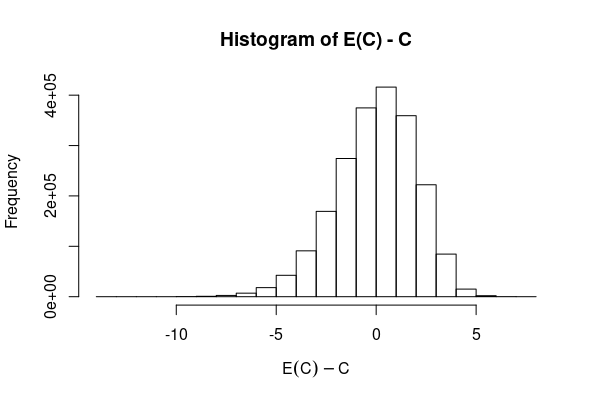
\includegraphics[scale=0.5]{images/labelling_histogram.png}
  \caption{Histogram of the difference between the expected number of vertices
    assigned each label and the actual number (for all labelled graphs)}
  \label{figure:labelling_histogram}
\end{figure}

%TODO: could insert an example.
The publications associated with the database \cite{foggia2001-2, DBLP:journals/prl/SantoFSV03}
say nothing about how the labels are distributed among the $N$ values. We
calculate the number of vertices that were assigned each label for each graph
(represented by $C$) and compare those values with the numbers we would expect
from a uniform distribution (represented by $E(C)$). We plot a histogram of the
difference $E(C) - C$ in Figure \ref{figure:labelling_histogram} and observe
that the difference is normally distributed around 0.

\section{Unlabelled graphs} \label{sec:unlabelled}
We also include a collection of benchmark instances for the subgraph isomorphism
problem\footnote{\url{http://liris.cnrs.fr/csolnon/SIP.html}} (with the
biochemical reactions dataset excluded since we are not dealing with directed
graphs). It contains only unlabelled graphs and consists of the following sets:

\begin{description}
\item[images-CVIU11] Graphs generated from segmented images. 43 pattern graphs
  and 146 target graphs, giving a total of \num{6278} instances.
\item[meshes-CVIU11] Graphs generated from meshes modelling 3D
  objects. 6 pattern graphs and 503 target graphs, giving a total of \num{3018}
  instances. Both \texttt{images-CVIU11} and \texttt{meshes-CVIU11} datasets are
  described in \cite{DBLP:journals/cviu/DamiandSHJS11}.
\item[images-PR15] Graphs generated from segmented images
  \cite{DBLP:journals/pr/SolnonDHJ15}. 24 pattern graphs and a single target
  graph, giving 24 instances.
\item[LV] Graphs with various properties (connected, biconnected, triconnected,
  bipartite, planar, etc.). 49 graphs are paired up in all possible ways, giving
  $49^2=\num{2401}$ instances.
\item[scalefree] Scale-free networks generated using a power law distribution of
  degrees (100 instances).
\item[si] Bounded valence graphs, 4D meshes, and randomly generated graphs
  (\num{1170} instances). This is the unlabelled part of the ARG database.
  \texttt{LV}, \texttt{scalefree}, and \texttt{si} datasets are described in
  \cite{DBLP:journals/ai/Solnon10, DBLP:journals/constraints/ZampelliDS10}.
\item[phase] Random graphs generated to be close to the
  satisfiable-unsatisfiable phase transition (200 instances)
  \cite{DBLP:conf/ijcai/McCreeshPT16}.
\item[largerGraphs] Larger instances of the \texttt{LV} dataset. There are 70
  graphs, giving $70^2=\num{4900}$ instances. The separation was made and used
  in \cite{DBLP:conf/aaai/HoffmannMR17, DBLP:conf/lion/KotthoffMS16,
    DBLP:conf/ijcai/McCreeshPT17}.
\end{description}

\begin{remark}
This set of instances was taken from the
repository\footnote{\url{https://github.com/jamestrimble/ijcai2017-partitioning-common-subgraph}}
for the \textsc{McSplit} paper \cite{DBLP:conf/ijcai/McCreeshPT17} and has some
minor differences from the version on Christine Solnon's website.
\end{remark}

\begin{remark}
  Since $k\downarrow$ comes from the subgraph isomorphism problem background, it
  treats the two (pattern and target) graphs differently. Therefore, when graphs
  are not divided into patterns and targets, we run the algorithms with both
  orders ($(G_1, G_2)$ and $(G_2, G_1)$).
\end{remark}

\chapter{Features}
%TODO: formulas for features?
The initial set of features is based on the algorithm selection paper for the
subgraph isomorphism problem \cite{DBLP:conf/lion/KotthoffMS16} and consists of
the following:

\begin{enumerate}
\item number of vertices,
\item number of edges,
\item mean degree,
\item maximum degree,
\item density,
\item mean distance between all pairs of vertices,
\item maximum distance between all pairs of vertices,
\item standard deviation of degrees,
\item number of loops,
\item proportion of all vertex pairs that have a distance of at least 2, 3, and 4,
\item whether the graph is connected.
%\item uniformity of the distribution of edges.
\end{enumerate}

We exclude feature extraction running time as a viable feature by itself since
it would not provide any insight into what properties of the graph affect which
algorithm is likely to achieve the best performance. Since $k\downarrow$ and
$\textsc{McSplit}\downarrow$ both start by looking for (complete) subgraph
isomorphisms, they are likely to outperform other algorithms when both graphs
are very similar and the maximum common subgraph has (almost) as many vertices
as the smaller of the two graphs. Thus, for each feature $f$ in features 1--7
(excluding the rest to avoid division by 0), we also add a feature for the ratio
$\frac{f(G_p)}{f(G_t)}$, where $G_p$ and $G_t$ are the pattern and target
graphs, respectively.

We analyse three different types of labelling and treat them as separate problems:

\begin{itemize}
\item no labels,
\item vertex labels,
\item vertex and edge labels.
\end{itemize}
For the last two types, we add a feature corresponding to $p$ defined in
Definition \ref{def:percent_labelling} and collect data for the following values
of p: 50\%, 33\%, 25\%, 20\%, 15\%, 10\%, 5\%. The values correspond to having
about 2, 3, 4, 5, 10, and 20 vertices/edges with the same label on average,
respectively.

\section{Distributions of Features}

\begin{figure}
  \centering
  \begin{subfigure}[t]{0.49\textwidth}
    \centering
    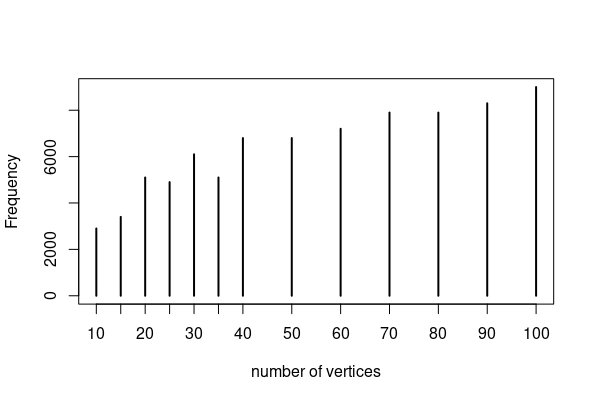
\includegraphics[width=\textwidth]{images/mcs_vertices.png}
  \end{subfigure}
  \begin{subfigure}[t]{0.49\textwidth}
    \centering
    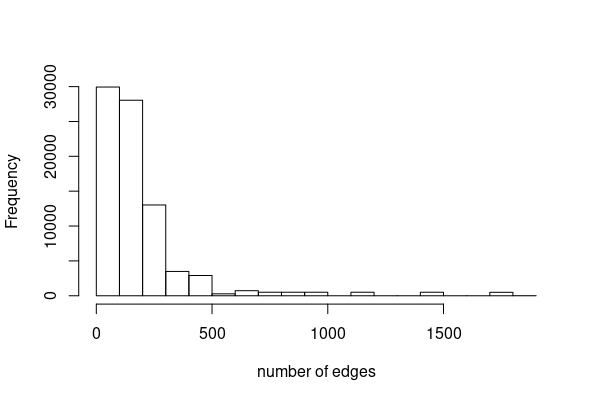
\includegraphics[width=\textwidth]{images/mcs_edges.png}
  \end{subfigure}
  \begin{subfigure}[t]{0.49\textwidth}
    \centering
    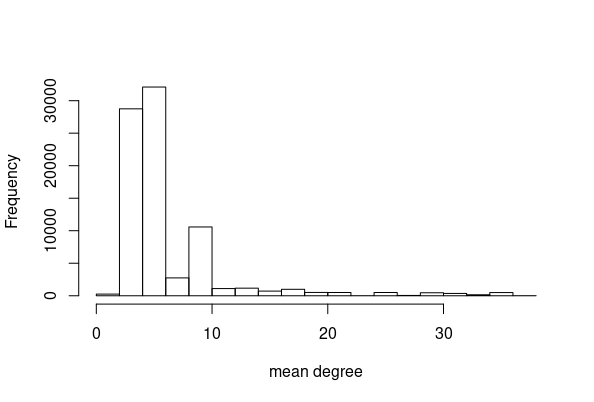
\includegraphics[width=\textwidth]{images/mcs_meandeg.png}
  \end{subfigure}
  \begin{subfigure}[t]{0.49\textwidth}
    \centering
    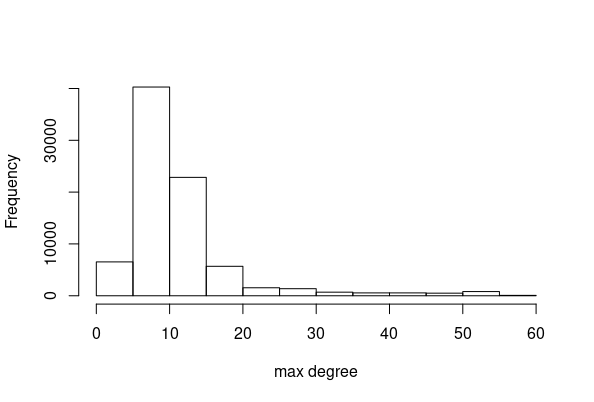
\includegraphics[width=\textwidth]{images/mcs_maxdeg.png}
  \end{subfigure}
  \begin{subfigure}[t]{0.49\textwidth}
    \centering
    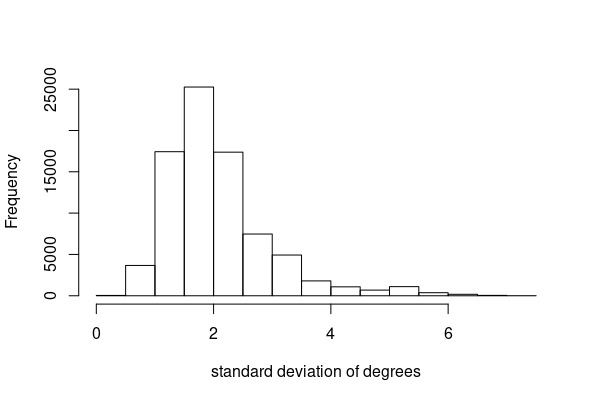
\includegraphics[width=\textwidth]{images/mcs_stddeg.png}
  \end{subfigure}
  \begin{subfigure}[t]{0.49\textwidth}
    \centering
    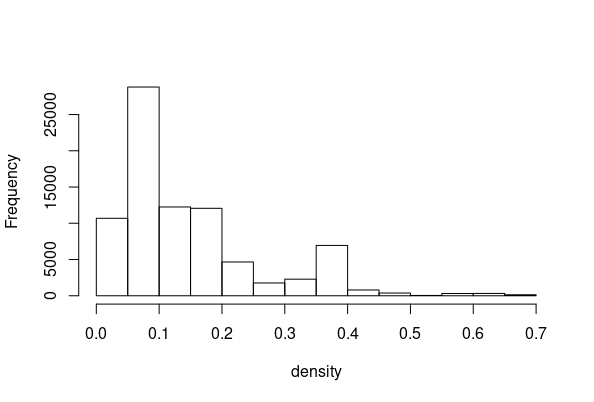
\includegraphics[width=\textwidth]{images/mcs_density.png}
  \end{subfigure}
  \begin{subfigure}[t]{0.49\textwidth}
    \centering
    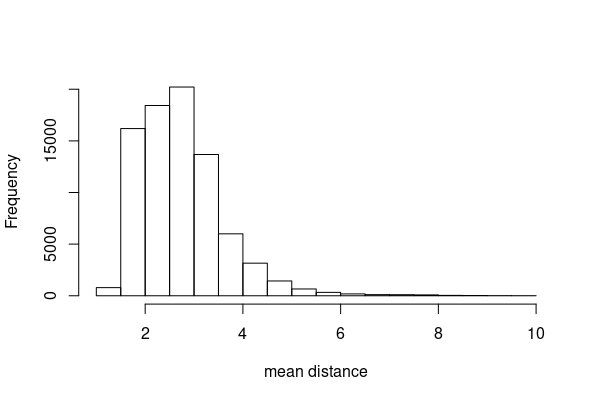
\includegraphics[width=\textwidth]{images/mcs_meandist.png}
  \end{subfigure}
  \begin{subfigure}[t]{0.49\textwidth}
    \centering
    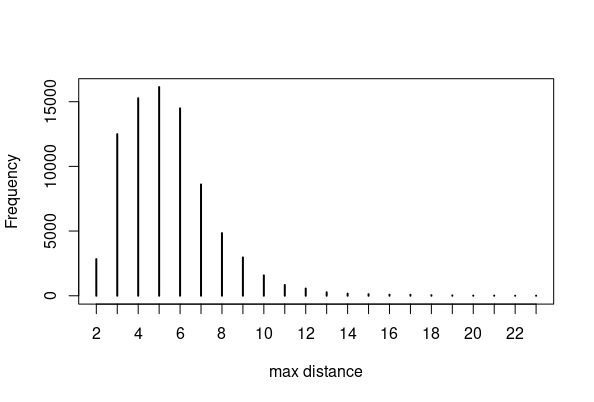
\includegraphics[width=\textwidth]{images/mcs_maxdist.png}
  \end{subfigure}
  \caption{Plots of how various features are distributed for the labelled graphs}
  \label{fig:mcs_features1}
\end{figure}

\begin{figure}
  \centering
  \begin{subfigure}[t]{0.49\textwidth}
    \centering
    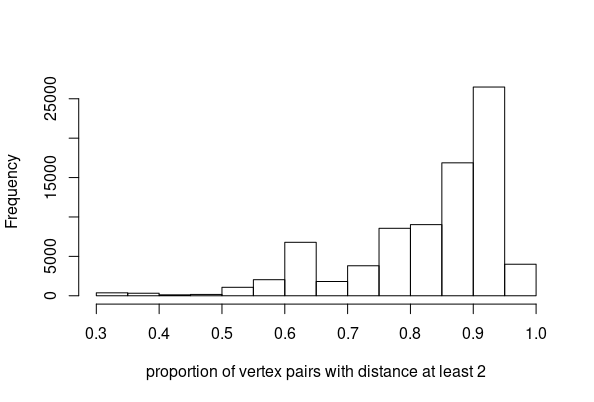
\includegraphics[width=\textwidth]{images/mcs_prop2.png}
  \end{subfigure}
  \begin{subfigure}[t]{0.49\textwidth}
    \centering
    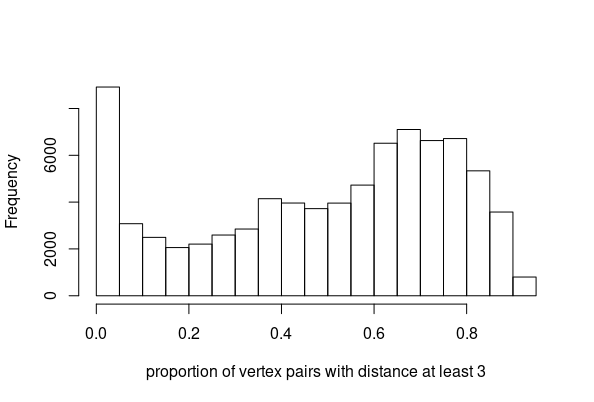
\includegraphics[width=\textwidth]{images/mcs_prop3.png}
  \end{subfigure}
  \begin{subfigure}[t]{0.49\textwidth}
    \centering
    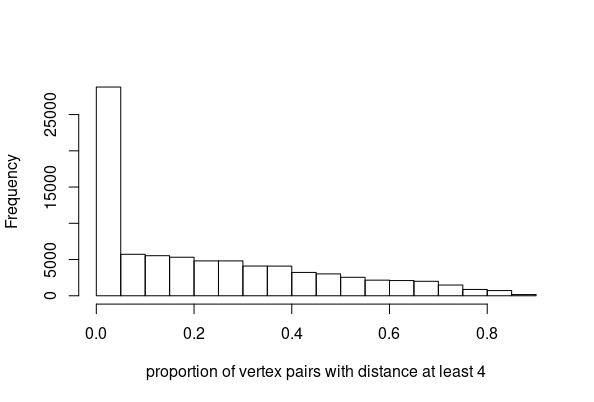
\includegraphics[width=\textwidth]{images/mcs_prop4.png}
  \end{subfigure}
  \caption{Plots showing typical distances between pairs of vertices for the
    labelled graphs}
  \label{fig:mcs_features2}
\end{figure}

\begin{figure}
  \centering
  \begin{subfigure}[t]{0.49\textwidth}
    \centering
    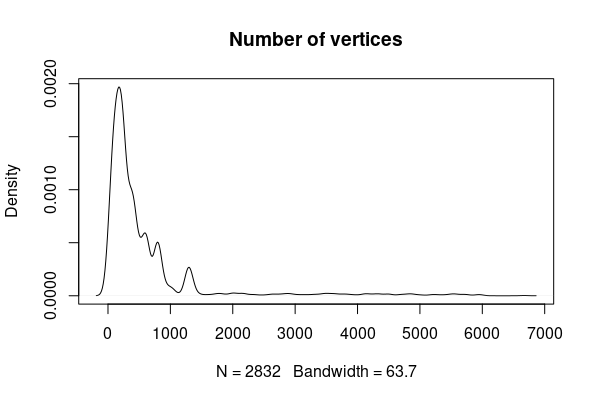
\includegraphics[width=\textwidth]{images/sip_vertices.png}
  \end{subfigure}
  \begin{subfigure}[t]{0.49\textwidth}
    \centering
    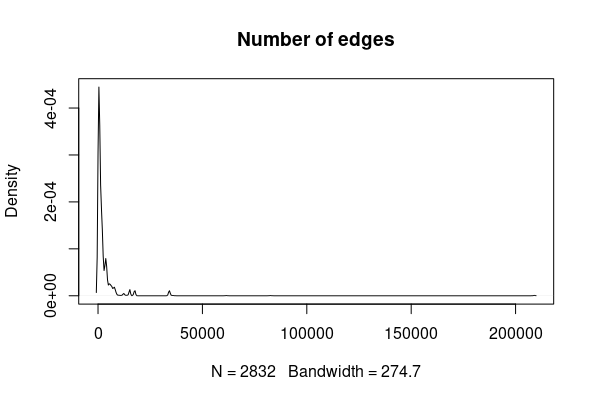
\includegraphics[width=\textwidth]{images/sip_edges.png}
  \end{subfigure}
  \begin{subfigure}[t]{0.49\textwidth}
    \centering
    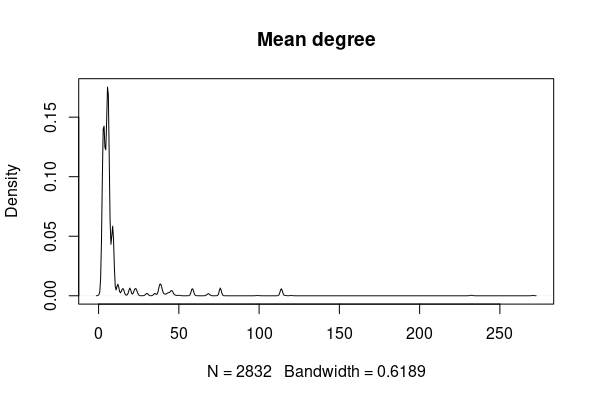
\includegraphics[width=\textwidth]{images/sip_meandeg.png}
  \end{subfigure}
  \begin{subfigure}[t]{0.49\textwidth}
    \centering
    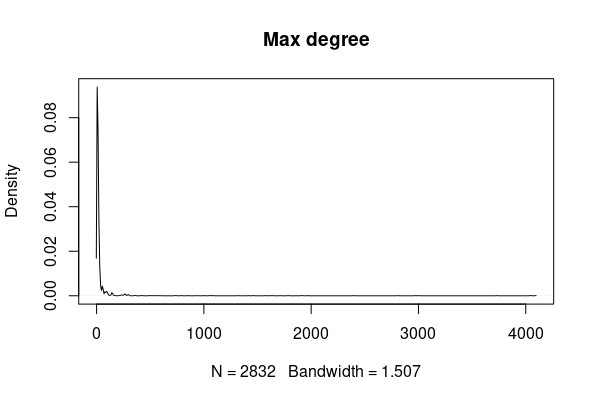
\includegraphics[width=\textwidth]{images/sip_maxdeg.png}
  \end{subfigure}
  \begin{subfigure}[t]{0.49\textwidth}
    \centering
    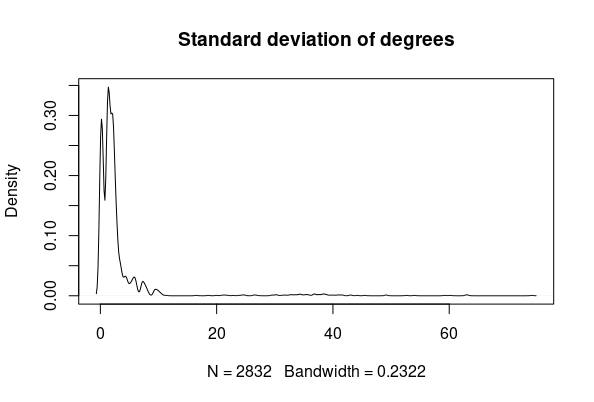
\includegraphics[width=\textwidth]{images/sip_stddeg.png}
  \end{subfigure}
  \begin{subfigure}[t]{0.49\textwidth}
    \centering
    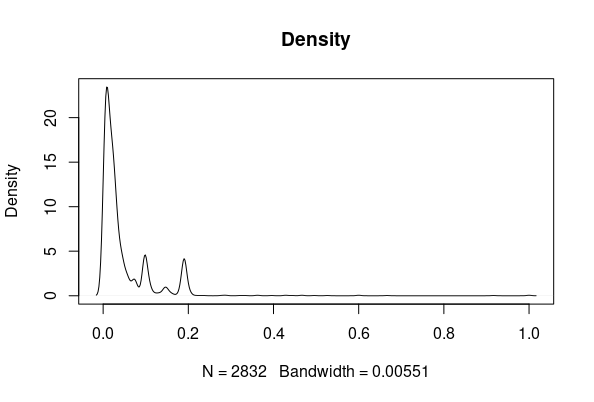
\includegraphics[width=\textwidth]{images/sip_density.png}
  \end{subfigure}
  \begin{subfigure}[t]{0.49\textwidth}
    \centering
    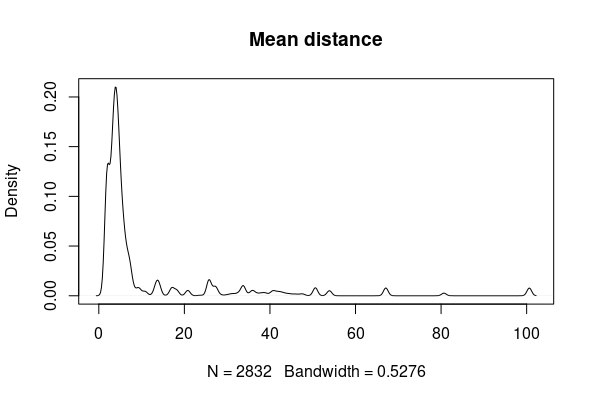
\includegraphics[width=\textwidth]{images/sip_meandist.png}
  \end{subfigure}
  \begin{subfigure}[t]{0.49\textwidth}
    \centering
    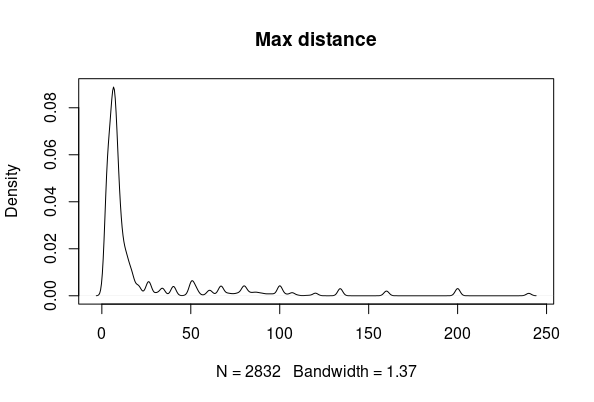
\includegraphics[width=\textwidth]{images/sip_maxdist.png}
  \end{subfigure}
  \caption{Plots of how various features are distributed for the unlabelled
    graphs}
  \label{fig:sip_features1}
\end{figure}

\begin{figure}
  \centering
  \begin{subfigure}[t]{0.49\textwidth}
    \centering
    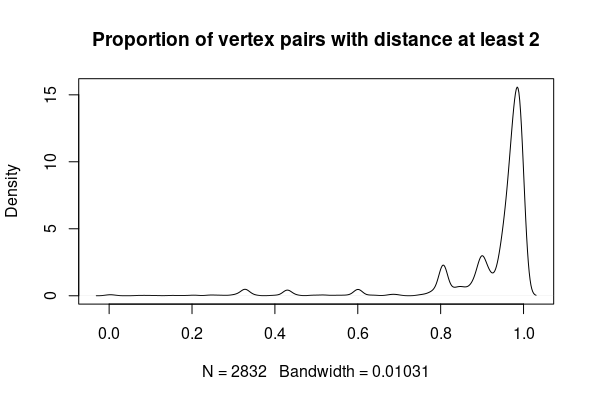
\includegraphics[width=\textwidth]{images/sip_prop2.png}
  \end{subfigure}
  \begin{subfigure}[t]{0.49\textwidth}
    \centering
    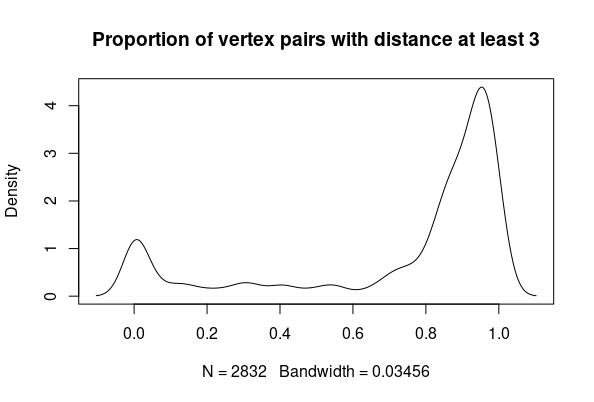
\includegraphics[width=\textwidth]{images/sip_prop3.png}
  \end{subfigure}
  \begin{subfigure}[t]{0.49\textwidth}
    \centering
    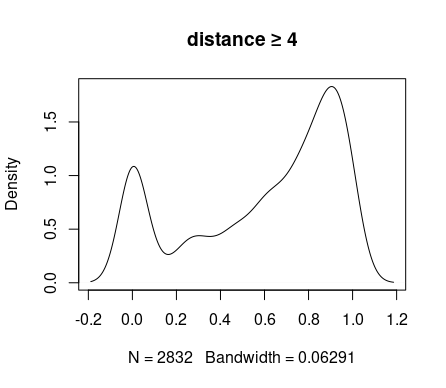
\includegraphics[width=\textwidth]{images/sip_prop4.png}
  \end{subfigure}
  \begin{subfigure}[t]{0.49\textwidth}
    \centering
    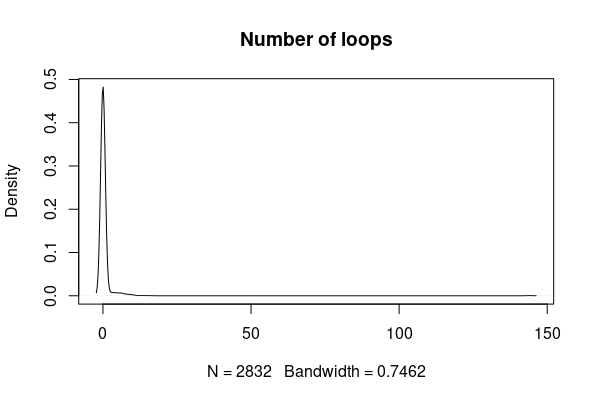
\includegraphics[width=\textwidth]{images/sip_loops.png}
  \end{subfigure}
  \caption{Plots showing typical distances between pairs of vertices and the
    number of loops for the unlabelled graphs}
  \label{fig:sip_features2}
\end{figure}

\begin{figure}
  \centering
  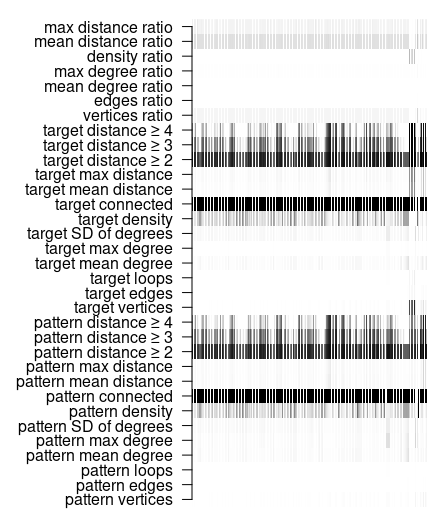
\includegraphics{images/features_heatmap.png}
  \caption{A heatmap for normalised features with black denoting the maximum
    value and white denoting the minimum for each feature}
  \label{fig:features_heatmap}
\end{figure}

%TODO: investigate feature correlation?
In this section we plot and discuss how the selected features are distributed in
different datasets. Most of the data is plotted, except for the number of loops
of the labelled dataset and connectedness of both labelled and unlabelled data.
For connectedness, 99.81\% of the labelled graphs are connected, compared to
93.19\% of the unlabelled graphs. As both numbers are quite high, they may not
be ideal for establishing if connectedness is a significant factor in
determining which algorithm performs the best, however, the numbers seem quite
representative of real data, where connected graphs are a lot more common. In
fact, applications in chemistry are often only interested in connected graphs
\cite{WCMS:WCMS5}.

With the labelled graphs, all graphs are assigned into pairs (A and B) with no
significant differences between them. Thus all of the statistical information is
provided only for pattern graphs and is plotted in Figures
\ref{fig:mcs_features1} and \ref{fig:mcs_features2}. As the number of loops
varies between two values, it is not plotted: 0.98\% of the graphs have a
single loop, other graphs have no loops. Other than the plot for number of
vertices, which is manually chosen by the creators of the database, all the
distributions in Figure \ref{fig:mcs_features1} are centered around lower
values, with some instances providing significantly higher values. More
importantly, we have some graphs that are quite dense and some graphs with
higher mean distance values.

For unlabelled graphs, we will only consider graphs that are part of a pair of
graphs solved by at least one algorithm. Since most of the data is heavily
skewed, Figures \ref{fig:sip_features1} and \ref{fig:sip_features2} show the
distributions as density plots. Because of this choice of which graphs to
include, all of the easy instances are solved and thus end up in the sample,
while only some of the harder instances are solved by at least one algorithm.
Harder instances typically have more vertices, which means they are also capable
of higher values for many other features, hence all of the density plots in
Figure \ref{fig:sip_features1} are right skewed. The same applies to the number
of loops in Figure \ref{fig:sip_features2}: almost all graphs have a small
number of them, while some (presumably larger) graphs have significantly more.
The same story is represented in the heatmap in Figure
\ref{fig:features_heatmap}, where the average values are coloured grey, largest
values black, and smallest values white. The rows that look almost completely
white represent features that have several significantly higher values.
% TODO: the heatmap is for both, not just SIP

To sum up, even though the distributions are far from normal, most of them still
provide a good range of different values. There is one important difference
between the plots of proportions of vertex pairs with distance $\ge k$ for $k =
2, 3, 4$ for labelled and unlabelled datasets (in Figures
\ref{fig:mcs_features2} and \ref{fig:sip_features2}, respectively). With
labelled graphs, the mean value keeps shifting to the left, while with
unlabelled graphs, the plot for $k = 4$ still has its highest peak around 0.9,
which means adding features for $k \ge 5$ could be valuable.

\chapter{Machine Learning}
After running the algorithms on all of the data for different types of labelling
and $p$ values, a machine learning (ML) algorithm can be trained to predict which
algorithm should be chosen for each pair of graphs. For that we are using an R
package called \textsc{Llama} \cite{kotthoff_llama_2013}, which was created for
exactly this purpose. For each pair of graphs it takes:

\begin{itemize}
\item A list of features. We treat the features of pattern and target graphs
  separately, giving more than 20 features per problem instance.
\item A list of performance measures for all algorithms, i.e., the values that
  we are trying to optimise. In this case (as in most cases), this corresponds
  to running time. The values are capped at the timeout value (1,000,000 ms).
  Furthermore, instances that were not run on the clique algorithm are also set
  to the timeout value. Finally, we filter out instances where all of the
  algorithms timed out.
\item A list of boolean values, denoting whether each algorithm successfully
  finished or not. Timeouts, the clique algorithm running out of memory, and
  instances that were not run with the clique algorithm because of their size
  are all marked as false.
\item A dataframe, measuring the running time taken to compute each feature for
  each problem instance. Alternatively, a single number for the approximate time
  taken to compute all features for any instance. This parameter is taken into
  account when comparing the algorithm portfolio against specific algorithms. As
  the main goal of this work is to gain insight about how the algorithms compare
  rather than to prove an algorithm portfolio as a superior approach, this
  parameter is not used.
\end{itemize}

After constructing the required dataframes as described above, the data needs to
be split into training and test sets. We use a technique called 10-fold
\emph{cross-validation}, which splits the data into 10 parts \cite{citeulike:1304145}.
9/10\textsuperscript{ths} of the data is used to train the ML algorithm, while
the remaining 1/10\textsuperscript{th} is used to evaluate how good the trained
model is. This process of training and evaluation is repeated 10 times, letting
each of the 10 parts be used for evaluation exactly once. The goodness-of-fit
criteria are then averaged out between the 10 runs.

The 10 folds could, of course, be chosen completely randomly. However, research
suggests that stratified cross-validation typically outperforms
random-sampling-based cross-validation and results in a better model
\cite{DBLP:conf/ijcai/Kohavi95}. Suppose we have a dataset of $N$ elements.
\emph{Stratified sampling} partitions it into a number of subpopulations $s_1,
\dots, s_n$ with $n_1, \dots, n_N$ elements, respectively (typically based on
the value of some feature or collection of features). It then draws from each
subpopulation independently, ensuring that approximately $n_i/N$ of the sample
comes from subpopulation $s_i$ for $i = 1, \dots, n$ \cite{lohr2009sampling}. In
this case the data is partitioned into four groups based on which algorithm
performed the best.

% TODO: describe/cite random forest
The cross-validation folds are then passed to the ML algorithm. We are using a
classifier called random forest as it is recommended in the manual
\cite{kotthoff_llama_2013} and successfully used in a similar study
\cite{DBLP:conf/lion/KotthoffMS16}.

As we are trying to use hundreds of megabytes of data, the R code was optimised
to reduce memory consumption by removing temporary variables as soon as they are
no longer needed and parallelised with the help of the \texttt{parallelMap}
package.

\section{Unlabelled Graphs}

\begin{figure}
  \centering
  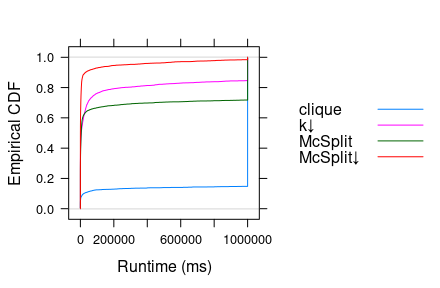
\includegraphics{images/ecdf_sip.png}
  \caption{Comparison of the runtimes of algorithms for the unlabelled dataset}
  \label{fig:ecdf_sip}
\end{figure}

\begin{figure}
  \centering
  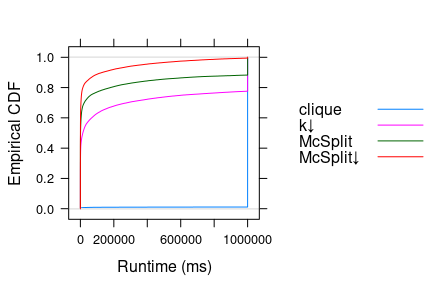
\includegraphics{images/ecdf_unlabelled.png}
  \caption{Comparison of the runtimes of algorithms for all of the unlabelled data}
  \label{fig:ecdf_unlabelled}
\end{figure}

\begin{figure}
  \centering
  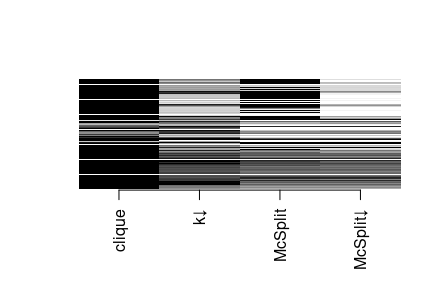
\includegraphics{images/runtime_heatmap.png}
  \caption{A heatmap of $\log_{10}$ runtimes: light colours for low running
    times and black for timing out}
  \label{fig:runtime_heatmap}
\end{figure}

In order to compare the runtimes of the algorithms, we use empirical cumulative
distribution function (ECDF) plots \cite{10.2307/2334448}: for each unit of time
on the $x$ axis, the $y$ value represents what part of the problem instances
was solved in that amount of time or less. Figures (TODO: add the MCS figure)
and \ref{fig:ecdf_sip} show the ECDF plots for unlabelled instances described in
Sections \ref{sec:labelled} and \ref{sec:unlabelled}, respectively. We can check
that the ordering of the algorithms in these plots is the same as in Figures
3.(a) and 4 in the \textsc{McSplit} paper \cite{DBLP:conf/ijcai/McCreeshPT17}.
Next, Figure \ref{fig:ecdf_unlabelled} provides the same plot for all of the
unlabelled data and Figure \ref{fig:runtime_heatmap} compares the runtimes of
the algorithms on a per-instance basis. Out of \num{45465} instances that were
solved by at least one algorithm, the clique encoding won 85 times,
$k\downarrow$ won 81 times, \textsc{McSplit} won \num{15017} times, and
$\textsc{McSplit}\downarrow$ won \num{21484} times. In the remaining 8798 cases
2 or more algorithms performed equally well (usually with a runtime of less than
10 ms). Note that even though $k\downarrow$ performs considerably better than
the clique encoding according to Figures \ref{fig:ecdf_unlabelled} and
\ref{fig:runtime_heatmap}, it is the best algorithm in only 81 instances, less
than the clique encoding. Given this information, we would expect the ML
algorithm to suggest using \textsc{McSplit} and $\textsc{McSplit}\downarrow$
most of the time, only suggesting $k\downarrow$ and the clique encoding in very
specific situations.

\section{Vertex-Labelled Graphs}

\section{Vertex- and Edge-Labelled Graphs}

%\begin{appendices}
%\end{appendices}

\bibliographystyle{plain}
\bibliography{references}
\end{document}
